\documentclass[11pt]{article}
\usepackage[utf8]{inputenc}
\usepackage[T1]{fontenc}
\usepackage{lmodern}
\usepackage[margin=1in]{geometry}
\usepackage{microtype}
\usepackage{graphicx}
\usepackage{booktabs}
\usepackage{array}
\usepackage{tabularx}
\usepackage{longtable}
\usepackage{float}
\usepackage{placeins}
\usepackage{xcolor}
\usepackage{caption}
\usepackage{natbib}
\usepackage[hidelinks]{hyperref}
\usepackage{fancyhdr}
\setlength{\parindent}{0pt}
\setlength{\parskip}{0.65em}
\setlength{\headheight}{14.5pt}
\renewcommand{\arraystretch}{1.15}
\definecolor{ink}{HTML}{19324A}
\definecolor{accent}{HTML}{A64B2A}
\hypersetup{colorlinks=true,linkcolor=ink,citecolor=accent,urlcolor=accent}
\pagestyle{fancy}
\fancyhf{}
\lhead{Chile: when did the external constraint bind?}
\rhead{v7}
\cfoot{\thepage}
\title{\textbf{When Did Chile's Balance-of-Payments Constraint Bind?}\\
\large An import-requirement account of machinery accumulation and external adjustment, 1920--2024}
\author{Chapter 2 research pipeline}
\date{29 July 2026}
\begin{document}
\maketitle

\begin{abstract}
Chile's imports are observed. The level of imports the country's productive structure required is not: it has to be estimated. This report estimates that requirement as a long-run relation between real imports, the gross machinery stock, non-reinvested surplus and the real exchange rate, and asks whether the gap between actual and required imports dates the years when the balance-of-payments constraint bound. A single long-run relation is found in all three samples. It is usable in two of them. Over 1920--2024 imports close 31\% of the gap each year and after 1974 they close 69\%, so the gap measures something imports respond to. Before 1973 they do not respond at all, and the relation carries no import requirement in that period. Where the measure works it dates 18 binding years over the century, concentrated in the 1930s, the 1950s, and the two post-reform adjustments of 1975--77 and 1983--86. It does not date 1961, the one crisis independently documented \citep{bcch2025}, because in 1961 imports stood above their required level rather than below it. The measure identifies the compression that follows an external crisis, not the over-absorption that precedes one.

\vspace{0.5em}\noindent\textbf{Keywords:} Chile; balance of payments; imports; machinery accumulation; real exchange rate; cointegration; error correction; Kaldor; Thirlwall
\end{abstract}

\FloatBarrier
\section{The question, and what has to be estimated to answer it}

Chile's industrialization ran on imported machinery. Building productive capacity meant buying capital goods abroad, and paying for them depended on export earnings and on access to external finance \citep{bcch2025,alvarez2003}. When those ran short, the imports that carried the accumulation had to be cut. The question is when that happened.

Answering it requires distinguishing two things that are easy to conflate. Actual imports are recorded in the national accounts every year. The level of imports the productive structure \emph{required} is not recorded anywhere; it is a relation that has to be estimated. Only once that required level exists can a shortfall be defined, and only a shortfall can indicate that the external constraint was doing the cutting.

Kaldor's mechanism supplies the reason machinery belongs at the centre of that relation: manufacturing expansion raises productivity and draws in the capital goods that carry it \citep{kaldor1967,kaldor1970}. Thirlwall's closure supplies the constraint: sustained growth is limited by export earnings and the import intensity of output, with external finance able to postpone but not remove the limit \citep{thirlwall1979,thirlwall1982,morenobrid2003}.

The required level is estimated as a long-run relation among four variables, all in logs. Writing imports as $m$, the machinery stock as $k$, non-reinvested surplus as $s$ and the real exchange rate as $r$:
\begin{equation}
m = \beta_1 k + \beta_2 s + \beta_3 r + c
\end{equation}
and the gap in a given year is $m - (\beta_1 k + \beta_2 s + \beta_3 r + c)$. A negative gap means imports sat below the level the relation implies. In the surplus approach $\beta_1$ is the foreign-exchange cost of the intensive margin of accumulation: how much import capacity a larger machinery stock commits the economy to, conditional on distribution and the relative price of foreign goods.

Throughout, a rise in the real exchange rate means real depreciation. The convention is confirmed in the data: the largest annual increases fall in 1932, 1956--57, 1974--75 and 1983--85, each a documented Chilean devaluation \citep{ffd1983a,ffd2002}.

\FloatBarrier
\section{Data}

Every estimate uses the frozen release \texttt{chile\_bop\_binding\_v1\_1}: 105 annual observations, 1920 to 2024, with 54 years before 1974 and 51 after. No stage re-queries a source or rebuilds a variable. Real series are in 2003 Chilean pesos, matching the GDP source so no rebasing is applied. The real exchange rate splices a ClioLab index through 2010 to the Banco Central series from 2011, rebased to the 2003 scale.

\begin{table}[H]
\centering
\caption{Provenance and the real-exchange-rate splice audit}
\begin{tabular}{p{6.0cm}p{2.4cm}p{5.6cm}}
\toprule
\textbf{Audit object} & \textbf{Result} & \textbf{Reading} \\
\midrule
Price base, all real series & 2003 CLP & Matches the GDP source; no rebasing applied. \\
Level correlation over 1986--2010 & 0.825 & The two sources move together. \\
Growth correlation over 1987--2010 & 0.750 & Year-to-year movement is shared. \\
Median absolute level gap & 9.34\% & They differ in level; this is a limitation. \\
2011 boundary change & 0.133 log points & Within four overlap-growth standard deviations. \\
Annual coverage & 105 years & One observation per year, 1920--2024. \\
\bottomrule
\end{tabular}
\end{table}

\begin{figure}[H]
\centering
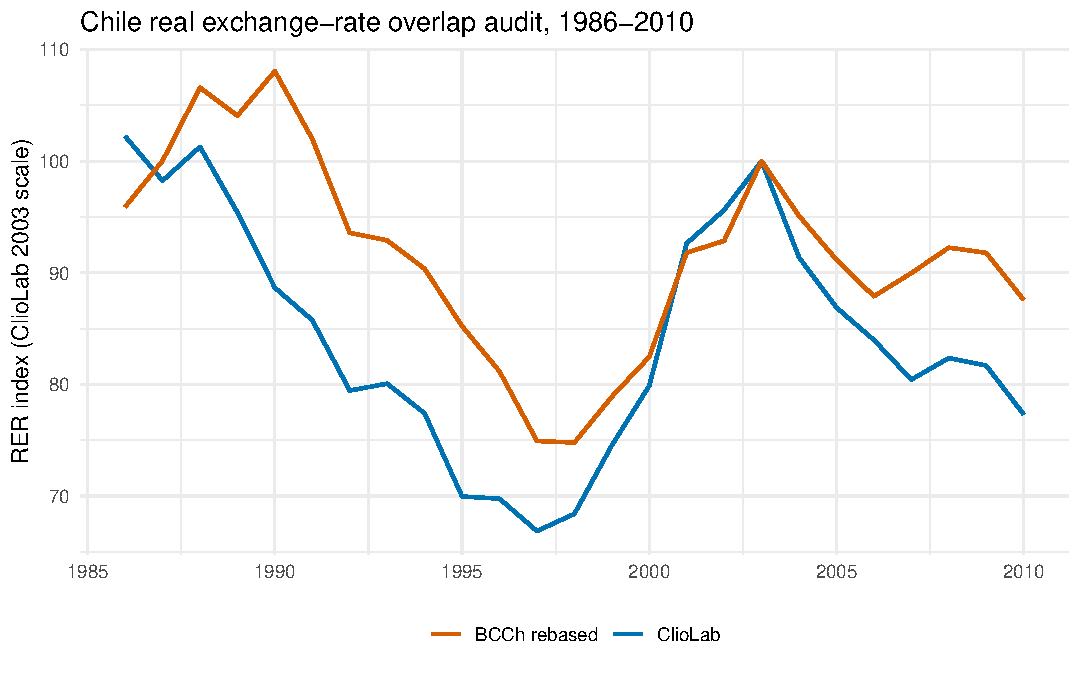
\includegraphics[width=0.90\textwidth]{figures/rer_overlap.pdf}
\caption{The two real-exchange-rate sources over their overlap. They move together over 1986--2010 while differing in level, which is why the splice is audited rather than assumed.}
\end{figure}

\begin{figure}[H]
\centering
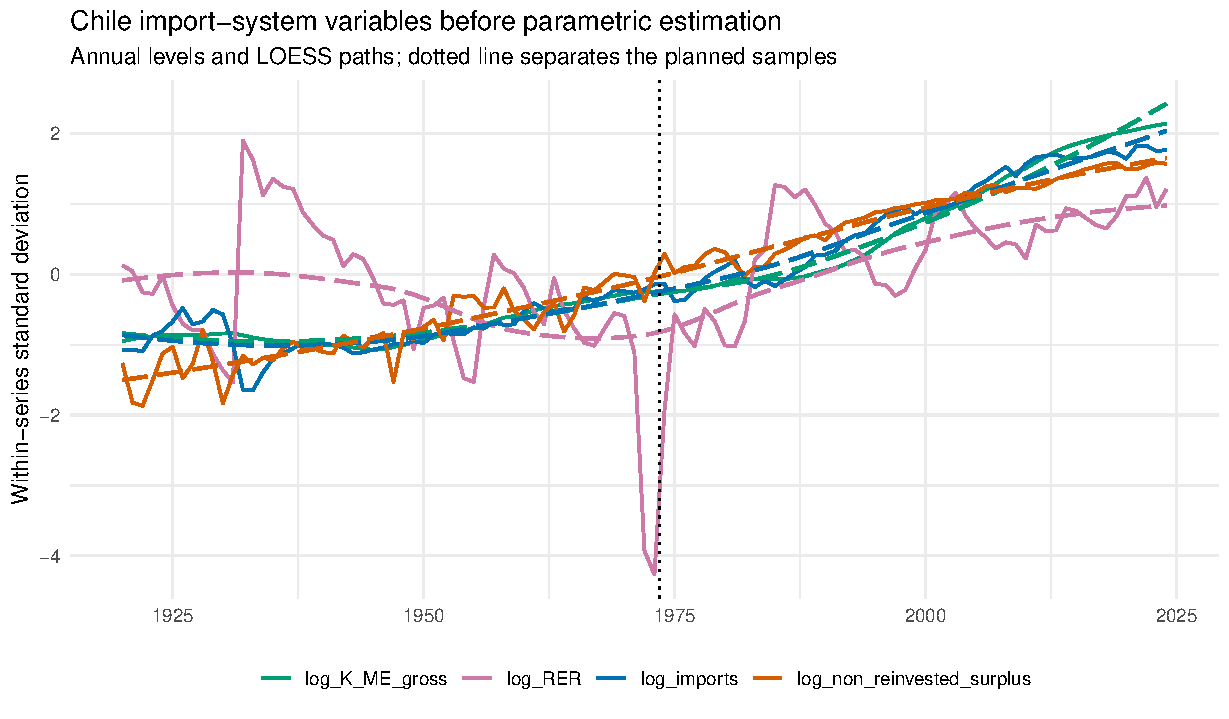
\includegraphics[width=0.94\textwidth]{figures/raw_system.pdf}
\caption{The four series with local trend lines, before any model is imposed. Imports and the machinery stock rise together across the century, with the two post-1974 accelerations visible without estimation.}
\end{figure}

\FloatBarrier
\section{How persistent is each series?}

A long-run relation between levels only makes sense if the levels themselves wander in a particular way. A series is integrated of order one, written I(1), when its level wanders without returning to any fixed value but its year-to-year change does settle down. Cointegration analysis is built for that case. Each variable is therefore tested before any system is estimated, on the level, then the change, then the change in the change, stopping at the first order where the series settles.

Three tests are used because they ask the question from opposite directions. Augmented Dickey--Fuller and Phillips--Perron start from the assumption that the series wanders and look for evidence against it, so a statistic more negative than the critical value is evidence of stationarity. KPSS starts from the opposite assumption, so a statistic \emph{above} its critical value is evidence of wandering. Agreement across all three makes a verdict safe; disagreement is reported as disagreement.

\begin{table}[H]
\centering
\caption{Test statistics against 5\% critical values, drift specification}
\footnotesize
\begin{tabular}{p{1.9cm}p{2.6cm}p{1.1cm}rrrrrp{2.0cm}}
\toprule
\textbf{Sample} & \textbf{Variable} & \textbf{Diffs} & \textbf{ADF} & \textbf{5\%} & \textbf{PP} & \textbf{KPSS} & \textbf{5\%} & \textbf{Verdict} \\
\midrule
1920--2024 & machinery stock & 0 & 0.59 & -2.88 & 3.34 & 1.960 & 0.463 & not stationary \\
1920--2024 & machinery stock & 1 & -2.29 & -2.88 & -2.09 & 1.115 & 0.463 & not stationary \\
1920--2024 & machinery stock & 2 & -7.57 & -2.88 & -8.95 & 0.072 & 0.463 & stationary \\
1920--2024 & real exchange rate & 0 & -2.69 & -2.88 & -3.06 & 0.467 & 0.463 & not stationary \\
1920--2024 & real exchange rate & 1 & -8.83 & -2.88 & -8.94 & 0.052 & 0.463 & stationary \\
1920--2024 & real imports & 0 & 0.29 & -2.88 & 0.14 & 2.030 & 0.463 & not stationary \\
1920--2024 & real imports & 1 & -7.81 & -2.88 & -7.53 & 0.151 & 0.463 & stationary \\
1920--2024 & non-reinvested surplus & 0 & -0.33 & -2.88 & -0.34 & 2.179 & 0.463 & not stationary \\
1920--2024 & non-reinvested surplus & 1 & -4.75 & -2.88 & -15.34 & 0.055 & 0.463 & stationary \\
1920--2024 & wage share & 0 & -1.35 & -2.88 & -2.61 & 1.721 & 0.463 & not stationary \\
1920--1973 & machinery stock & 0 & -0.86 & -2.89 & 1.22 & 1.009 & 0.463 & not stationary \\
1920--1973 & machinery stock & 1 & -1.81 & -2.89 & -1.81 & 0.615 & 0.463 & not stationary \\
1920--1973 & machinery stock & 2 & -5.05 & -2.89 & -6.38 & 0.138 & 0.463 & stationary \\
1920--1973 & real exchange rate & 0 & -1.48 & -2.89 & -1.16 & 0.529 & 0.463 & not stationary \\
1920--1973 & real exchange rate & 1 & -5.03 & -2.89 & -6.69 & 0.200 & 0.463 & stationary \\
1920--1973 & real imports & 0 & -0.97 & -2.89 & -1.26 & 0.816 & 0.463 & not stationary \\
1920--1973 & real imports & 1 & -5.57 & -2.89 & -4.93 & 0.087 & 0.463 & stationary \\
1920--1973 & non-reinvested surplus & 0 & -1.05 & -2.89 & -1.45 & 1.314 & 0.463 & not stationary \\
1920--1973 & wage share & 0 & -4.53 & -2.89 & -4.98 & 0.055 & 0.463 & stationary \\
1974--2024 & machinery stock & 0 & -0.99 & -2.89 & 0.91 & 1.349 & 0.463 & not stationary \\
1974--2024 & machinery stock & 1 & -1.92 & -2.93 & -1.99 & 0.417 & 0.463 & not stationary \\
1974--2024 & machinery stock & 2 & -5.11 & -2.93 & -6.05 & 0.182 & 0.463 & stationary \\
1974--2024 & real exchange rate & 0 & -3.24 & -2.89 & -3.29 & 0.677 & 0.463 & not stationary \\
1974--2024 & real exchange rate & 1 & -3.70 & -2.93 & -7.85 & 0.154 & 0.463 & stationary \\
1974--2024 & real imports & 0 & -1.08 & -2.89 & -0.58 & 1.342 & 0.463 & not stationary \\
1974--2024 & real imports & 1 & -3.77 & -2.93 & -6.96 & 0.103 & 0.463 & stationary \\
1974--2024 & non-reinvested surplus & 0 & -1.08 & -2.89 & -0.35 & 1.328 & 0.463 & not stationary \\
1974--2024 & non-reinvested surplus & 1 & -4.95 & -2.93 & -7.50 & 0.093 & 0.463 & stationary \\
1974--2024 & wage share & 0 & -1.26 & -2.89 & -1.65 & 1.062 & 0.463 & not stationary \\
\bottomrule
\end{tabular}
\end{table}

\begin{table}[H]
\centering
\caption{Order of integration and what follows for each variable}
\begin{tabular}{p{2.1cm}p{3.4cm}p{2.2cm}p{6.0cm}}
\toprule
\textbf{Sample} & \textbf{Series} & \textbf{Order} & \textbf{Disposition} \\
\midrule
1920--2024 & machinery stock & I(2) & break aware or exploratory route required \\
1920--2024 & real exchange rate & I(1) & cointegrating state candidate \\
1920--2024 & real imports & I(1) & cointegrating state candidate \\
1920--2024 & non-reinvested surplus & I(1) & cointegrating state candidate \\
1920--2024 & wage share & unresolved by d3 & break aware or exploratory route required \\
1920--1973 & machinery stock & I(2) & break aware or exploratory route required \\
1920--1973 & real exchange rate & I(1) & cointegrating state candidate \\
1920--1973 & real imports & I(1) & cointegrating state candidate \\
1920--1973 & non-reinvested surplus & I(0) & stationary control candidate \\
1920--1973 & wage share & I(0) & stationary control candidate \\
1974--2024 & machinery stock & I(2) & break aware or exploratory route required \\
1974--2024 & real exchange rate & I(1) & cointegrating state candidate \\
1974--2024 & real imports & I(1) & cointegrating state candidate \\
1974--2024 & non-reinvested surplus & I(1) & cointegrating state candidate \\
1974--2024 & wage share & I(0) & stationary control candidate \\
\bottomrule
\end{tabular}
\end{table}

Read variable by variable. \textbf{Real imports} settle after one difference in every sample: the level wanders, the growth rate does not. Imports enter the long-run relation without qualification. \textbf{The real exchange rate} behaves the same way in all three samples. \textbf{Non-reinvested surplus} is I(1) over the century and after 1974, but before 1973 it is already stationary in levels, so in that sample it contributes no long-run wandering for the others to be tied to. \textbf{The wage share} $\omega_t$ is stationary before and after 1974 and unresolved over the full span, so it never enters as a long-run variable and appears only in a robustness specification. \textbf{The machinery stock} $K^{ME}$ is the problem, and it needs its own section.

One cell is genuinely inconclusive and is not smoothed over. For the change in the machinery stock over the full sample under a trend specification, KPSS returns 0.090 against a 5\% value of 0.146, which does not reject stability, while ADF returns -2.76 against -3.43, which does not reject wandering. The two point opposite ways once a trend is allowed. The verdict rests on the drift specification, where all three tests agree, and the disagreement is recorded rather than resolved by preference.

\FloatBarrier
\section{Why a machinery stock can need two differences}

The machinery stock needs two differences before it settles, in every sample. That is unusual enough to explain from the ground up, because it is the single biggest constraint on everything that follows.

\subsection*{Start with what a capital stock is}

A capital stock is a running total. This year's machinery is last year's machinery, minus what wore out, plus what was newly installed:
\begin{equation}
K_t = (1 - z) K_{t-1} + I_t
\end{equation}
where $I_t$ is machinery investment during the year and $z$ is the fraction of the existing stock retired. Nothing here is a modelling choice; it is how the stock is built from investment flows.

Now ask what happens if investment itself has no level it returns to. Suppose investment drifts upward for two decades, settles at a higher pace, then drifts again, never reverting to a long-run average. Adding up a series that wanders gives a total that wanders more. And because $z$ is small for machinery, very little of the past is discarded each year, so almost the whole history stays in the total. The running total inherits the wandering of the flow and adds its own on top.

\subsection*{What the two differences mean}

Saying the machinery stock is I(2) says exactly this: not only does the \emph{level} of the stock fail to return to any fixed value, its \emph{growth rate} fails to as well. The rate of machinery accumulation itself moves to a new level and stays there. Only the change in the growth rate settles down.

\subsection*{What the tests show}

In levels, ADF returns 0.59 against a 5\% value of -2.88 and KPSS returns 1.960 against 0.463: the level wanders and both tests agree. After one difference---looking at the growth rate of the stock rather than its level---ADF still returns only -2.29 against -2.88 and KPSS still returns 1.115 against 0.463. The growth rate is no more settled than the level was. Only after a second difference does the picture change decisively: ADF -7.57, Phillips--Perron -8.95, KPSS 0.072---all three agree on stationarity.

\subsection*{What it costs}

Standard cointegration analysis assumes every variable in the long-run relation needs the same single difference to settle. Putting an I(2) variable alongside I(1) variables makes the relation \emph{unbalanced}: the two sides wander at different orders, and a coefficient estimated on them is not a long-run elasticity in the usual sense. The honest options are machinery growth in place of the stock, methods built for I(2) systems, or keeping the levels specification and reporting the limitation. This report keeps the levels specification, because the machinery stock is the variable the mechanism is about, and carries the limitation forward explicitly. A differenced-machinery specification is estimated alongside it as a check.

\subsection*{What it means about Chile}

The statistic describes something concrete. Chile's machinery stock did not merely grow across the century---the pace at which it grew shifted and stayed shifted, averaging 2.1\% a year before 1973 and 7.4\% after. A series whose growth rate steps up to a new level and remains there is precisely what a second unit root describes. The awkward statistical property and the post-reform transformation of Chilean accumulation are the same fact seen from two directions \citep{ffd2002,solimano2024}.

\FloatBarrier
\section{How many long-run relations are there?}

With the variables classified, the next question is how many independent long-run relations tie them together. The answer is the \emph{rank}: zero means no relation and the variables drift apart permanently; one means a single relation holds them together; more than one means several do. Rank is estimated with the Johansen trace test, which asks in sequence whether the number of relations is zero, then at most one, and so on, stopping at the first hypothesis it cannot reject.

Rather than test one preferred model, the relation is built up one variable at a time, so the evidence reads as a sequence.

\begin{table}[H]
\centering
\caption{The specifications, from the mechanism core outward}
\footnotesize
\begin{tabular}{p{1.4cm}p{6.2cm}p{6.4cm}}
\toprule
\textbf{Rung} & \textbf{Variables} & \textbf{What it adds} \\
\midrule
M1 & real imports, machinery stock & Kaldor core: imports and machinery accumulation \\
M2 & real imports, machinery stock, non-reinvested surplus & adds the surplus not internally recapitalized \\
M3 & real imports, machinery stock, non-reinvested surplus, real exchange rate & headline: Kaldor controlled by the real exchange rate \\
M4 & real imports, machinery stock, non-reinvested surplus, wage share & robustness: legacy fourth variable in place of the RER \\
M3d & real imports, machinery growth, non-reinvested surplus, real exchange rate & balanced-order diagnostic: machinery enters in first differences \\
\bottomrule
\end{tabular}
\end{table}

\begin{table}[H]
\centering
\caption{Number of long-run relations at each rung, constant and two lags}
\begin{tabular}{p{2.2cm}p{1.6cm}p{2.4cm}p{3.4cm}p{3.4cm}}
\toprule
\textbf{Sample} & \textbf{Rung} & \textbf{Relations} & \textbf{Residual-correlation} $p$ & \textbf{Same order throughout?} \\
\midrule
1920--2024 & M1 & 1 & 0.883 & no \\
1920--2024 & M2 & 1 & 0.032 & no \\
1920--2024 & M3 & 1 & 0.035 & no \\
1920--2024 & M3d & 2 & 0.301 & yes \\
1920--2024 & M4 & 1 & 0.076 & no \\
1920--1973 & M1 & 0 & n/a & no \\
1920--1973 & M2 & 0 & n/a & no \\
1920--1973 & M3 & 1 & 0.532 & no \\
1920--1973 & M3d & 1 & 0.831 & no \\
1920--1973 & M4 & 1 & 0.911 & no \\
1974--2024 & M1 & 1 & 0.723 & no \\
1974--2024 & M2 & 1 & 0.979 & no \\
1974--2024 & M3 & 1 & 0.927 & no \\
1974--2024 & M3d & 1 & 0.932 & yes \\
1974--2024 & M4 & 1 & 0.802 & no \\
\bottomrule
\end{tabular}
\end{table}

The sequence tells a clear story. Over the full century and after 1974, a single relation appears as soon as imports and machinery are put together, and it survives every addition. Before 1973 the two- and three-variable systems find nothing: no relation ties imports to machinery, or to machinery and surplus, in the pre-reform period. A relation appears only once the real exchange rate is added. That is the first sign the pre-1973 system behaves differently, and Section~\ref{sec:alpha} shows why it matters.

\begin{table}[H]
\centering
\caption{The four-variable relation across deterministic terms and lags}
\begin{tabular}{p{2.2cm}p{1.9cm}p{1.1cm}p{1.9cm}p{2.6cm}p{2.6cm}}
\toprule
\textbf{Sample} & \textbf{Determ.} & \textbf{Lags} & \textbf{Relations} & \textbf{Resid.\ corr.\ } $p$ & \textbf{Largest non-unit root} \\
\midrule
1920--2024 & const & 2 & 1 & 0.035 & 0.716 \\
1920--2024 & const & 3 & 1 & 0.452 & 0.866 \\
1920--2024 & trend & 2 & 2 & 0.522 & 0.841 \\
1920--2024 & trend & 3 & 1 & 0.368 & 0.866 \\
1920--1973 & const & 2 & 1 & 0.532 & 0.763 \\
1920--1973 & const & 3 & 1 & 0.951 & 0.823 \\
1920--1973 & trend & 2 & 2 & 0.951 & 0.763 \\
1920--1973 & trend & 3 & 1 & 0.804 & 0.823 \\
1974--2024 & const & 2 & 1 & 0.927 & 0.682 \\
1974--2024 & const & 3 & 1 & 0.688 & 0.798 \\
1974--2024 & trend & 2 & 0 & n/a & n/a \\
1974--2024 & trend & 3 & 1 & 0.741 & 0.798 \\
\bottomrule
\end{tabular}
\end{table}

The specification carried forward in each sample finds exactly one relation, leaves no residual correlation at 5\%, and has stable dynamics. Requiring exactly one matters: when the test finds two, the single relation extracted from a two-dimensional space is one arbitrary combination of the two and cannot be read as \emph{the} import requirement. The last column is the stability check. A system tied together by one relation among four variables must carry three permanent trends, so three roots sit on the unit circle by construction; the question is whether the remaining roots lie inside it. They do, between 0.68 and 0.84.

\begin{figure}[H]
\centering
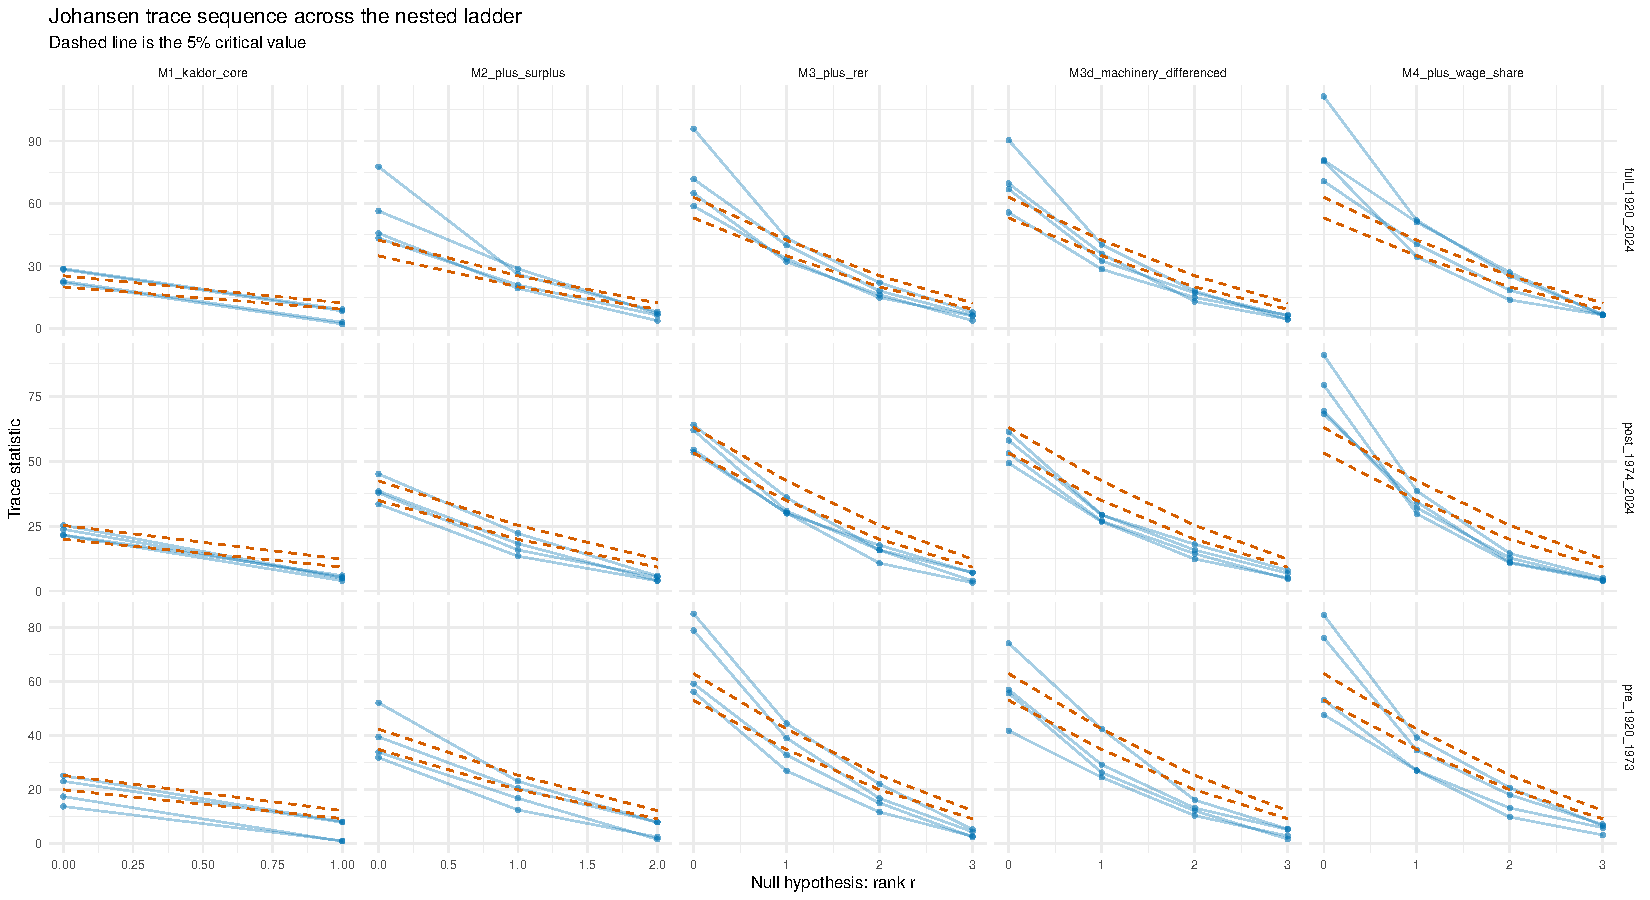
\includegraphics[width=0.97\textwidth]{figures/rank_grid.pdf}
\caption{Trace statistics across every rung and sample against the 5\% critical value (dashed). Where the solid line starts above the dashed one and then crosses below, that crossing is the number of relations.}
\end{figure}

\FloatBarrier
\section{What the long-run relation says}

\begin{table}[H]
\centering
\caption{The estimated import requirement}
\begin{tabular}{p{2.2cm}p{3.6cm}p{2.4cm}p{3.0cm}p{2.6cm}}
\toprule
\textbf{Sample} & \textbf{Variable} & \textbf{Coefficient} & \textbf{Import share} & \textbf{Elasticity?} \\
\midrule
1920--2024 & real imports & 1.000 & 0.747 & yes \\
1920--2024 & machinery stock & 0.578 & 0.747 & yes \\
1920--2024 & non-reinvested surplus & 0.393 & 0.747 & yes \\
1920--2024 & real exchange rate & 0.551 & 0.747 & yes \\
1920--1973 & real imports & 1.000 & 0.042 & no \\
1920--1973 & machinery stock & 11.661 & 0.042 & no \\
1920--1973 & non-reinvested surplus & -7.055 & 0.042 & no \\
1920--1973 & real exchange rate & 19.738 & 0.042 & no \\
1974--2024 & real imports & 1.000 & 0.808 & yes \\
1974--2024 & machinery stock & 0.683 & 0.808 & yes \\
1974--2024 & non-reinvested surplus & 0.177 & 0.808 & yes \\
1974--2024 & real exchange rate & 0.187 & 0.808 & yes \\
\bottomrule
\multicolumn{5}{p{15.5cm}}{\footnotesize The import share is the weight imports carry in the estimated relation. Normalizing on imports divides through by it, so a small share makes the reported coefficients arithmetic artifacts rather than elasticities.} \\
\end{tabular}
\end{table}

Over the full century the required import level rises by 0.58\% for every 1\% increase in the machinery stock, and after 1974 by 0.68\%. Read through the surplus approach this is the foreign-exchange commitment attached to the intensive margin of accumulation: enlarging the machinery stock obliges the economy to sustain a proportionally higher level of imports.

The pre-1973 column cannot be read this way. Before 1973 imports carry only 0.042 of the weight in the relation, so normalizing on imports divides by something close to zero, and the resulting numbers---a machinery coefficient above eleven, a real-exchange-rate coefficient near twenty---are an artifact of the arithmetic. The relation found before 1973 is not an import relation. Section~\ref{sec:alpha} confirms this from an entirely separate direction.

The real exchange rate enters the long-run relation with a \textbf{positive} sign: 0.55 over the century and 0.19 after 1974. Since a rise means depreciation, a more depreciated currency goes with \emph{higher} required imports, the opposite of a relative-price brake. The pattern is in the raw data, not an artifact of the system: over 1920--2024 the correlation between the log real exchange rate and the goods-import share of GDP is 0.54. The reading that fits Chilean structure is that capital and intermediate imports are hard to substitute domestically, so depreciation raises their peso cost without displacing them, while depreciation episodes coincide with the external pressure that accompanies accumulation drives \citep{albala2006,palma2019}. Section~\ref{sec:gamma} shows the real exchange rate doing something quite different within the year.

\begin{table}[H]
\centering
\caption{The machinery coefficient beside two simpler comparisons}
\begin{tabular}{p{2.6cm}p{3.4cm}p{3.4cm}p{4.0cm}}
\toprule
\textbf{Sample} & \textbf{Long-run coefficient} & \textbf{Level slope} & \textbf{Growth-rate ratio} \\
\midrule
1920--2024 & 0.578 & 0.979 & 0.919 \\
1920--1973 & 11.661 & 1.109 & 1.320 \\
1974--2024 & 0.683 & 0.851 & 0.801 \\
\bottomrule
\end{tabular}
\end{table}

Two series that both trend upward will appear related whether or not anything ties them together, so the comparison matters. If the estimated coefficient simply reproduced the ratio of average growth rates it would be measuring shared drift. It does not: over the full century the long-run coefficient is 0.58 while the growth ratio is 0.92 and the level slope is 0.98. The system estimate sits well below both, which is what conditioning on surplus and the real exchange rate does.

\FloatBarrier
\section{Which variable does the adjusting, and which does not}
\label{sec:alpha}

A long-run relation says nothing on its own about who moves when it is violated. That is the adjustment coefficient: for each variable, the fraction of last year's gap closed this year. A coefficient indistinguishable from zero says that variable ignores the gap, which is weak exogeneity. For the question at hand this is the decisive test, because a gap only measures an import requirement if imports are what responds to it.

\begin{table}[H]
\centering
\caption{Adjustment to the long-run gap, by equation}
\begin{tabular}{p{2.2cm}p{3.6cm}p{2.2cm}rrp{3.0cm}}
\toprule
\textbf{Sample} & \textbf{Equation for} & \textbf{Coefficient} & \textbf{t} & \textbf{p} & \textbf{Responds?} \\
\midrule
1920--2024 & machinery stock & -0.010 & -1.36 & 0.178 & does not adjust \\
1920--2024 & real exchange rate & 0.123 & 1.98 & 0.051 & does not adjust \\
1920--2024 & real imports & -0.315 & -4.87 & 0.000 & adjusts \\
1920--2024 & non-reinvested surplus & -0.072 & -0.74 & 0.462 & does not adjust \\
1920--1973 & machinery stock & 0.002 & 4.02 & 0.000 & adjusts \\
1920--1973 & real exchange rate & 0.003 & 0.46 & 0.645 & does not adjust \\
1920--1973 & real imports & -0.005 & -0.71 & 0.479 & does not adjust \\
1920--1973 & non-reinvested surplus & -0.022 & -1.96 & 0.056 & does not adjust \\
1974--2024 & machinery stock & -0.026 & -0.75 & 0.458 & does not adjust \\
1974--2024 & real exchange rate & 0.068 & 0.48 & 0.637 & does not adjust \\
1974--2024 & real imports & -0.685 & -3.34 & 0.002 & adjusts \\
1974--2024 & non-reinvested surplus & -0.291 & -1.94 & 0.059 & does not adjust \\
\bottomrule
\end{tabular}
\end{table}

Over the full century imports carry the adjustment, closing 31\% of the gap each year with a t ratio of -4.87. After 1974 the response is far faster, 69\% within the year, and imports are the only variable responding significantly: the machinery stock, surplus and the real exchange rate all ignore the gap. That is the configuration the question needs. Imports absorb the disequilibrium and the other three push it around, so the gap is a genuine import requirement and the speed at which imports close it measures how hard the requirement bites.

Before 1973 the picture inverts. Imports respond by -0.005 with a t ratio of -0.71 and $p = 0.479$---indistinguishable from no response. The machinery stock is what adjusts, at a t ratio of 4.02. The relation that exists before 1973 is one machinery closes, not one imports close. This is the same conclusion the normalization diagnostic reached in the previous section, arrived at independently: before 1973 there is no import requirement for imports to fall short of. Under import-substituting industrialization capital-goods imports were administratively allocated through licensing and multiple exchange rates rather than adjusted to a price-and-quantity equilibrium, and a relation imports do not error-correct is what that arrangement looks like in the time series \citep{ffd2002,albala2006}.

\begin{figure}[H]
\centering
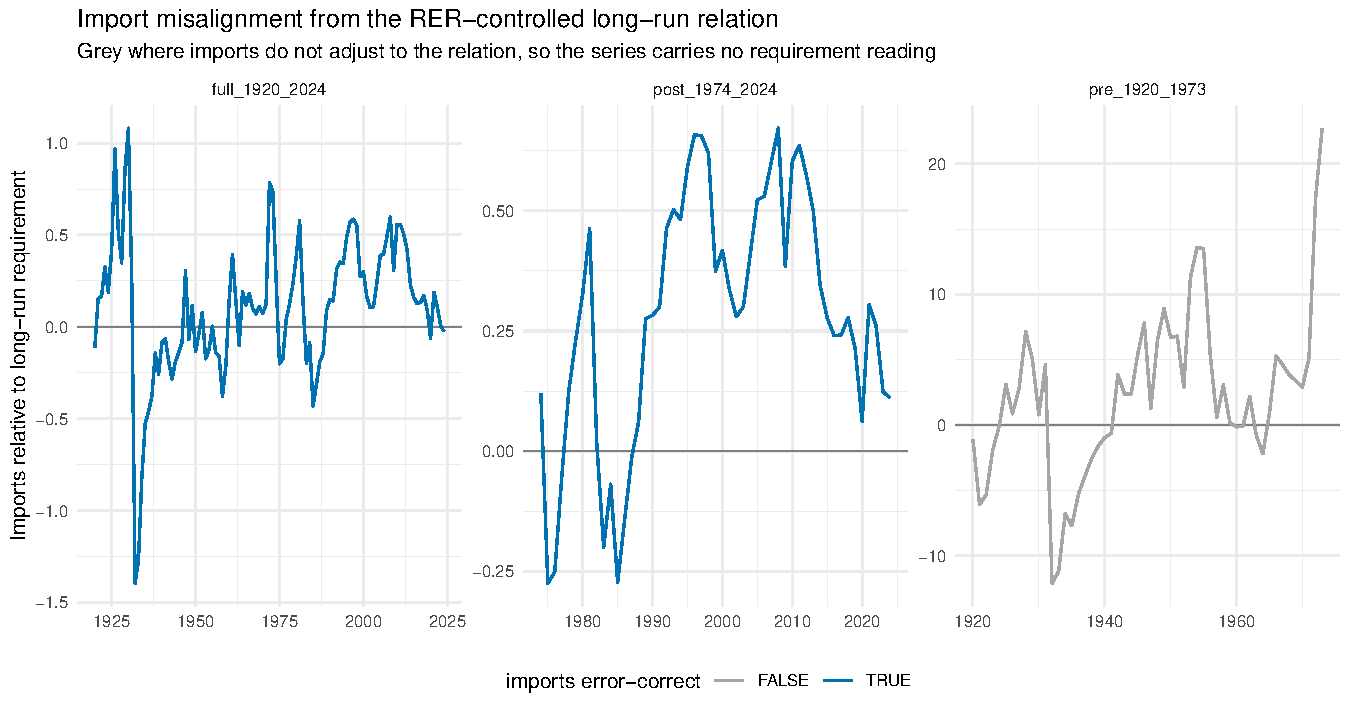
\includegraphics[width=0.92\textwidth]{figures/misalignment_usability.pdf}
\caption{The gap for each sample, greyed where imports do not respond to it. The pre-1973 line is drawn but carries no requirement reading.}
\end{figure}

\FloatBarrier
\section{What moves imports within the year}
\label{sec:gamma}

\begin{table}[H]
\centering
\caption{Short-run structure of the import equation}
\begin{tabular}{p{2.2cm}p{4.6cm}p{2.2cm}rrp{1.8cm}}
\toprule
\textbf{Sample} & \textbf{Term} & \textbf{Coefficient} & \textbf{t} & \textbf{p} & \textbf{Sig.\ 5\%} \\
\midrule
1920--2024 & change in machinery stock, lag 1 & -1.247 & -1.13 & 0.260 & no \\
1920--2024 & change in machinery stock, lag 2 & 2.499 & 2.41 & 0.018 & yes \\
1920--2024 & change in real exchange rate, lag 1 & -0.198 & -1.66 & 0.100 & no \\
1920--2024 & change in real exchange rate, lag 2 & -0.067 & -0.56 & 0.579 & no \\
1920--2024 & change in real imports, lag 1 & 0.437 & 3.73 & 0.000 & yes \\
1920--2024 & change in real imports, lag 2 & -0.066 & -0.63 & 0.530 & no \\
1920--2024 & change in non-reinvested surplus, lag 1 & 0.028 & 0.40 & 0.687 & no \\
1920--2024 & change in non-reinvested surplus, lag 2 & 0.067 & 1.05 & 0.298 & no \\
1920--1973 & change in machinery stock, lag 1 & 0.098 & 0.11 & 0.916 & no \\
1920--1973 & change in real exchange rate, lag 1 & 0.112 & 0.51 & 0.613 & no \\
1920--1973 & change in real imports, lag 1 & 0.427 & 2.66 & 0.011 & yes \\
1920--1973 & change in non-reinvested surplus, lag 1 & 0.127 & 1.42 & 0.161 & no \\
1974--2024 & change in machinery stock, lag 1 & 3.285 & 3.70 & 0.001 & yes \\
1974--2024 & change in real exchange rate, lag 1 & -0.320 & -1.45 & 0.155 & no \\
1974--2024 & change in real imports, lag 1 & 0.025 & 0.17 & 0.866 & no \\
1974--2024 & change in non-reinvested surplus, lag 1 & 0.586 & 3.19 & 0.003 & yes \\
\bottomrule
\end{tabular}
\end{table}

Over the full century imports have their own momentum: last year's import growth carries 0.44 into this year's, the most significant short-run term in the equation. After 1974 that momentum disappears---the own-lag coefficient falls to 0.025 and is indistinguishable from zero---and machinery growth takes over at 3.29 with a t ratio of 3.70, alongside non-reinvested surplus at 0.59. Post-reform import growth is driven by what is being installed and what surplus is available to finance it, not by its own past.

The real exchange rate is where short and long run part company. In the long-run relation its coefficient is positive. Within the year it enters negatively in every sample----0.198 over the century, $p = 0.100$, and -0.320 after 1974---so a depreciation does compress imports in the short term, though only marginally significantly. The relative price works as a brake on impact and as a co-mover over the long haul. Reporting only one of the two would misdescribe what the exchange rate does in this system.

Before 1973 nothing but the own lag matters: machinery growth, surplus and the real exchange rate are all insignificant in the import equation. The disconnection found in the previous section shows up here too.

\FloatBarrier
\section{The gap beside the external accounts}

The gap is a model quantity, so on its own it cannot establish that the external constraint was binding: a shortfall relative to an estimated requirement could reflect a mis-specified requirement. Independent evidence is needed, and it comes from the external accounts, which are observed rather than estimated.

A year is counted as binding only when two independent things agree---imports below the requirement the relation implies, \emph{and} at least one external-account indicator showing stress, meaning a current-account or goods deficit of 3\% of GDP or more, a fall in manufactured imports of at least 3 percentage points of GDP, or the financing indicator triggering. Years satisfying only one are recorded as satisfying only one. Nothing is counted as binding on the model alone.

\begin{table}[H]
\centering
\caption{What each category means}
\footnotesize
\begin{tabular}{p{4.4cm}p{10.4cm}}
\toprule
\textbf{Category} & \textbf{Meaning} \\
\midrule
binding confirmed & Imports sat below the level the long-run relation implies, and the external accounts showed stress in the same year. Both kinds of evidence agree. \\ \addlinespace
imports short only & Imports sat below the implied level, but no external-account indicator crossed its threshold. The model sees a shortfall the accounts do not corroborate. \\ \addlinespace
external stress only & The external accounts showed stress, but imports were at or above the level the relation implies. Pressure without an import shortfall. \\ \addlinespace
not binding & Neither imports fell short of the implied level nor did the accounts show stress. \\ \addlinespace
no estimate for year & The lag structure leaves this year without a value for the long-run relation, so no statement is made about it. \\ \addlinespace
external stress no usable model signal & The accounts showed stress, and in this sample the model provides no usable import signal because imports do not adjust to the relation. \\ \addlinespace
no stress no usable model signal & The accounts showed no stress, and in this sample the model provides no usable import signal. \\ \addlinespace
\bottomrule
\end{tabular}
\end{table}

\begin{figure}[H]
\centering
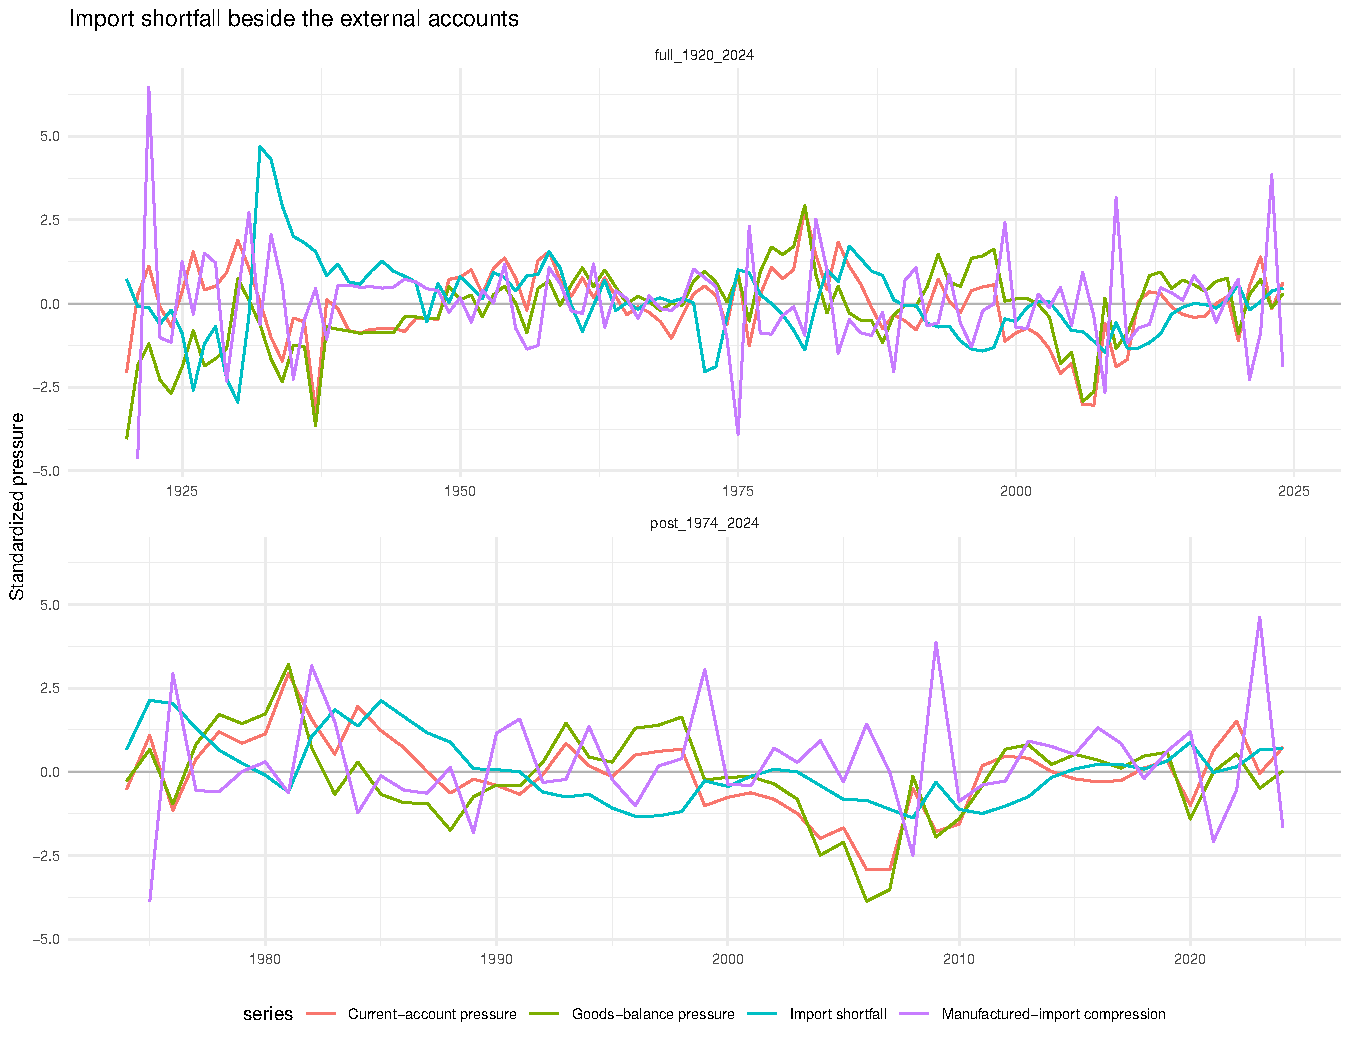
\includegraphics[width=0.92\textwidth]{figures/shortfall_vs_accounts.pdf}
\caption{The import shortfall and the three account-based pressure measures on one standardized scale. They rise together in the 1930s, the mid-1950s, and the mid-1970s and mid-1980s, and diverge in the early 1960s.}
\end{figure}

\begin{table}[H]
\centering
\caption{Years by category}
\begin{tabular}{p{2.6cm}p{1.8cm}p{3.0cm}p{2.8cm}p{1.8cm}p{1.4cm}}
\toprule
\textbf{Sample} & \textbf{Binding} & \textbf{Shortfall only} & \textbf{Stress only} & \textbf{Neither} & \textbf{Total} \\
\midrule
1920--2024 & 18 & 18 & 37 & 32 & 105 \\
1920--1973 & 0 & 0 & 30 & 24 & 54 \\
1974--2024 & 7 & 1 & 18 & 25 & 51 \\
\bottomrule
\end{tabular}
\end{table}

Every year of the release is accounted for in each sample. The pre-1973 row is not a finding about Chile: it records that in that sample the model supplies no usable import signal, so the confirmation rule can never be met. Thirty of those years show external stress in the accounts; what is missing is a requirement measure to pair it with, and the report does not convert that absence into a claim that the constraint never bound before 1973.

\begin{table}[H]
\centering
\caption{Binding episodes}
\begin{tabular}{p{2.8cm}p{2.4cm}p{2.0cm}p{2.2cm}p{2.6cm}}
\toprule
\textbf{Sample} & \textbf{Years} & \textbf{Length} & \textbf{Peak year} & \textbf{Peak pressure} \\
\midrule
1920--2024 & 1933 & 1 & 1933 & 1.627 \\
1920--2024 & 1937--1938 & 2 & 1938 & 0.041 \\
1920--2024 & 1950--1951 & 2 & 1950 & 0.570 \\
1920--2024 & 1953--1954 & 2 & 1954 & 0.963 \\
1920--2024 & 1957--1959 & 3 & 1958 & 1.323 \\
1920--2024 & 1963 & 1 & 1963 & 0.479 \\
1920--2024 & 1975--1976 & 2 & 1976 & 0.436 \\
1920--2024 & 1983--1986 & 4 & 1985 & 0.825 \\
1920--2024 & 2024 & 1 & 2024 & 0.004 \\
1974--2024 & 1975--1977 & 3 & 1976 & 0.970 \\
1974--2024 & 1983--1986 & 4 & 1983 & 1.073 \\
\bottomrule
\end{tabular}
\end{table}

\begin{figure}[H]
\centering
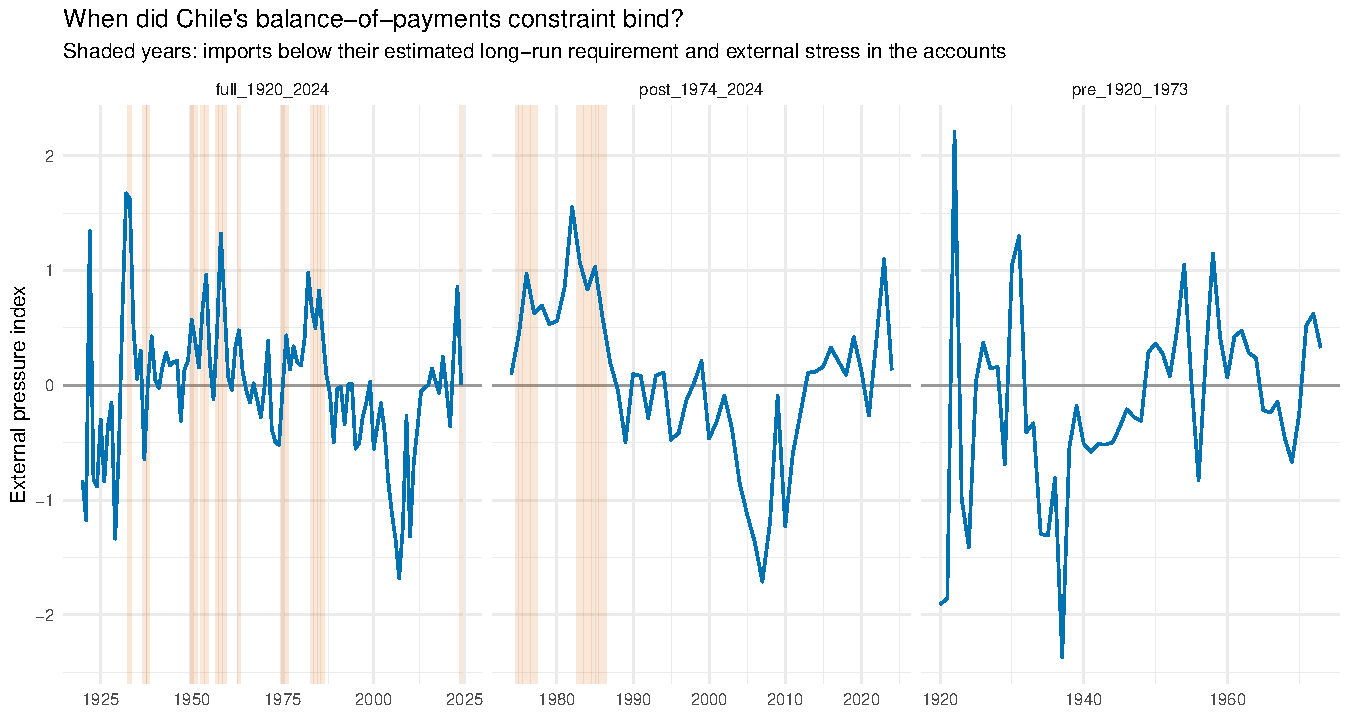
\includegraphics[width=0.92\textwidth]{figures/pressure_index.pdf}
\caption{The combined pressure index by sample, with binding years shaded. The tallest sustained blocks are the 1950s and the two post-reform adjustments.}
\end{figure}

The dated episodes line up with Chilean external history. 1933 sits in the Depression collapse of export earnings. The 1950--51, 1953--54 and 1957--59 runs fall inside the import-substituting decades, when capital-goods imports expanded against stagnant export receipts \citep{bcch2025}. 1975--77 follows the post-coup opening and the first oil shock, and 1983--86 is the debt crisis \citep{ffd1983a,ffd1983b}. Both post-reform episodes appear in the full-century and post-1974 datings alike, which is the strongest internal agreement in the report.

\FloatBarrier
\section{Does the gap identify when the constraint bound?}

Partly, and the qualification is specific enough to be useful. The gap identifies binding years where imports demonstrably respond to it, which means the full century and the post-1974 sample and not the decades before 1973. Where it works it is corroborated: 18 of the 105 years in the full sample show a shortfall and independent external stress together, and the episodes fall where Chilean external history puts them.

The decisive test is the one independent date available. The Banco Central's centennial history records the 1961 balance-of-payments crisis and the abandonment of the fixed exchange rate \citep{bcch2025}. The chronology does not identify it. In 1961 the gap is 0.394---imports stood \emph{above} their required level, the largest positive gap in the surrounding decade---while the external accounts did show stress. The year is recorded as external stress without an import shortfall.

That is a coherent economic reading rather than a failure to explain. The sequence around it is 1958 and 1959 below the requirement and confirmed binding, 1960 through 1962 above it with stress continuing, then 1963 below again. What 1961 looks like in this measure is an economy sustaining imports above what its productive structure and export earnings supported, financed by reserves and external credit until they ran out. The crisis was the exhaustion of that financing; the compression came afterwards. An import-shortfall measure registers the adjustment, not the over-absorption that made adjustment necessary \citep{thirlwall1982,morenobrid2003}.

So the measure dates \emph{external adjustment episodes} rather than crisis onsets, and that is what it should be used for. A chronology of when imports were compressed against a machinery-implied requirement is a different object from a chronology of when reserves ran out, and 1961 is where the two come apart most visibly.

\FloatBarrier
\section{Limitations}

\textbf{The machinery stock is I(2).} The promoted specification puts an I(2) variable in a levels relation with I(1) variables, so it is unbalanced and the machinery coefficient is not a long-run elasticity in the strict sense. A differenced-machinery specification is estimated as a check and finds a relation in every sample, but the levels version is what the report interprets. Resolving this properly means either a net-stock or investment-flow formulation or a method built for I(2) systems.

\textbf{Before 1973 the method does not apply.} Imports do not respond to the estimated relation and the relation does not normalize on imports. Both diagnostics point the same way, and the consequence is that the report has nothing to say about the timing of binding episodes in the import-substituting decades---the period the 1961 benchmark falls in.

\textbf{One external benchmark is a thin test.} The verified evidence base supplies exactly one precisely dated crisis, and no additional marker was invented to pad the comparison. The interpretation offered for the 1961 disagreement is plausible and is not established by a single case.

\textbf{The real exchange rate's long-run sign is unresolved.} A positive long-run coefficient on a depreciation measure cannot be read as a price elasticity. The short-run coefficient has the expected negative sign, which is reassuring but does not explain the long-run pattern.

\textbf{The splice is measurable.} The real exchange rate joins two sources with a median level gap of 9.34\%, which enters every specification that uses it.

\FloatBarrier
\section*{Data availability and reproducibility}

The frozen release is \texttt{data/releases/chile\_bop\_binding\_v1\_1/}. Every number is copied from a completed stage ledger; the builder performs no estimation. The SHA-256 hash of every consumed input is recorded in \texttt{output/CL/BOP\_BINDING\_V7/S99\_REPORT\_ASSEMBLY/}, and the staged ledgers sit in \texttt{data/} beside this file. Stage integrity ledgers for the estimation and dating stages both report every check passing, and the builder refuses to assemble if either fails. Each gap value was verified to reproduce the long-run relation for its own year, to a maximum absolute deviation of 3.5e-13.

The threshold model reported in the previous version is absent here. Its regime effect was not statistically supported, and the estimation stage refuses to run if any threshold ledger is among its inputs.

\textbf{Ethics.} The study uses historical aggregate data and involves no human subjects.

\textbf{AI-use disclosure.} Claude Code assisted with reproducible code, diagnostics, evidence organization and report assembly under human direction. All claims are auditable against the frozen release and the staged ledgers.

\FloatBarrier
\appendix
\section{Full integration-order battery}

\footnotesize
\begin{longtable}{p{1.6cm}p{3.4cm}p{0.6cm}p{1.1cm}p{0.6cm}rrrrr}
\toprule
\textbf{Sample} & \textbf{Variable} & \textbf{Diffs} & \textbf{Determ.} & \textbf{n} & \textbf{ADF} & \textbf{5\%} & \textbf{PP} & \textbf{KPSS} & \textbf{5\%} \\
\midrule
\endhead
1920--2024 & machinery stock & 0 & drift & 105 & 0.59 & -2.88 & 3.34 & 1.960 & 0.463 \\
1920--2024 & machinery stock & 0 & trend & 105 & -2.25 & -3.43 & -0.97 & 0.480 & 0.146 \\
1920--2024 & machinery stock & 1 & drift & 104 & -2.29 & -2.88 & -2.09 & 1.115 & 0.463 \\
1920--2024 & machinery stock & 1 & trend & 104 & -2.76 & -3.43 & -2.78 & 0.090 & 0.146 \\
1920--2024 & machinery stock & 2 & drift & 103 & -7.57 & -2.88 & -8.95 & 0.072 & 0.463 \\
1920--2024 & machinery stock & 2 & trend & 103 & -7.55 & -3.43 & -8.90 & 0.071 & 0.146 \\
1920--2024 & structures stock & 0 & drift & 105 & 0.23 & -2.88 & 0.61 & 2.179 & 0.463 \\
1920--2024 & structures stock & 0 & trend & 105 & -1.85 & -3.43 & -1.00 & 0.354 & 0.146 \\
1920--2024 & structures stock & 1 & drift & 104 & -3.51 & -2.88 & -3.90 & 0.203 & 0.463 \\
1920--2024 & structures stock & 1 & trend & 104 & -3.60 & -3.43 & -3.88 & 0.132 & 0.146 \\
1920--2024 & real exchange rate & 0 & drift & 105 & -2.69 & -2.88 & -3.06 & 0.467 & 0.463 \\
1920--2024 & real exchange rate & 0 & trend & 105 & -3.00 & -3.43 & -3.33 & 0.227 & 0.146 \\
1920--2024 & real exchange rate & 1 & drift & 104 & -8.83 & -2.88 & -8.94 & 0.052 & 0.463 \\
1920--2024 & real exchange rate & 1 & trend & 104 & -8.79 & -3.43 & -8.89 & 0.029 & 0.146 \\
1920--2024 & real imports & 0 & drift & 105 & 0.29 & -2.88 & 0.14 & 2.030 & 0.463 \\
1920--2024 & real imports & 0 & trend & 105 & -2.60 & -3.43 & -2.24 & 0.407 & 0.146 \\
1920--2024 & real imports & 1 & drift & 104 & -7.81 & -2.88 & -7.53 & 0.151 & 0.463 \\
1920--2024 & real imports & 1 & trend & 104 & -7.99 & -3.43 & -7.53 & 0.042 & 0.146 \\
1920--2024 & non-reinvested surplus & 0 & drift & 105 & -0.33 & -2.88 & -0.34 & 2.179 & 0.463 \\
1920--2024 & non-reinvested surplus & 0 & trend & 105 & -3.91 & -3.43 & -7.04 & 0.156 & 0.146 \\
1920--2024 & non-reinvested surplus & 1 & drift & 104 & -4.75 & -2.88 & -15.34 & 0.055 & 0.463 \\
1920--2024 & non-reinvested surplus & 1 & trend & 104 & -4.73 & -3.43 & -15.23 & 0.038 & 0.146 \\
1920--2024 & wage share & 0 & drift & 105 & -1.35 & -2.88 & -2.61 & 1.721 & 0.463 \\
1920--2024 & wage share & 0 & trend & 105 & -3.49 & -3.43 & -5.65 & 0.253 & 0.146 \\
1920--1973 & machinery stock & 0 & drift & 54 & -0.86 & -2.89 & 1.22 & 1.009 & 0.463 \\
1920--1973 & machinery stock & 0 & trend & 54 & -2.28 & -3.45 & -0.60 & 0.347 & 0.146 \\
1920--1973 & machinery stock & 1 & drift & 53 & -1.81 & -2.89 & -1.81 & 0.615 & 0.463 \\
1920--1973 & machinery stock & 1 & trend & 53 & -2.40 & -3.45 & -2.31 & 0.163 & 0.146 \\
1920--1973 & machinery stock & 2 & drift & 52 & -5.05 & -2.89 & -6.38 & 0.138 & 0.463 \\
1920--1973 & machinery stock & 2 & trend & 52 & -5.21 & -3.45 & -6.31 & 0.133 & 0.146 \\
1920--1973 & structures stock & 0 & drift & 54 & -1.18 & -2.89 & -1.12 & 1.412 & 0.463 \\
1920--1973 & structures stock & 0 & trend & 54 & -3.39 & -3.45 & -1.82 & 0.170 & 0.146 \\
1920--1973 & structures stock & 1 & drift & 53 & -2.48 & -2.89 & -2.66 & 0.223 & 0.463 \\
1920--1973 & structures stock & 1 & trend & 53 & -2.63 & -3.45 & -2.81 & 0.163 & 0.146 \\
1920--1973 & structures stock & 2 & drift & 52 & -5.20 & -2.89 & -8.24 & 0.087 & 0.463 \\
1920--1973 & structures stock & 2 & trend & 52 & -5.15 & -3.45 & -8.22 & 0.074 & 0.146 \\
1920--1973 & real exchange rate & 0 & drift & 54 & -1.48 & -2.89 & -1.16 & 0.529 & 0.463 \\
1920--1973 & real exchange rate & 0 & trend & 54 & -2.16 & -3.45 & -1.79 & 0.140 & 0.146 \\
1920--1973 & real exchange rate & 1 & drift & 53 & -5.03 & -2.89 & -6.69 & 0.200 & 0.463 \\
1920--1973 & real exchange rate & 1 & trend & 53 & -5.19 & -3.45 & -6.82 & 0.073 & 0.146 \\
1920--1973 & real imports & 0 & drift & 54 & -0.97 & -2.89 & -1.26 & 0.816 & 0.463 \\
1920--1973 & real imports & 0 & trend & 54 & -2.13 & -3.45 & -2.12 & 0.229 & 0.146 \\
1920--1973 & real imports & 1 & drift & 53 & -5.57 & -2.89 & -4.93 & 0.087 & 0.463 \\
1920--1973 & real imports & 1 & trend & 53 & -5.62 & -3.45 & -4.90 & 0.041 & 0.146 \\
1920--1973 & non-reinvested surplus & 0 & drift & 54 & -1.05 & -2.89 & -1.45 & 1.314 & 0.463 \\
1920--1973 & non-reinvested surplus & 0 & trend & 54 & -4.94 & -3.45 & -5.64 & 0.052 & 0.146 \\
1920--1973 & wage share & 0 & drift & 54 & -4.53 & -2.89 & -4.98 & 0.055 & 0.463 \\
1920--1973 & wage share & 0 & trend & 54 & -4.53 & -3.45 & -4.93 & 0.055 & 0.146 \\
1974--2024 & machinery stock & 0 & drift & 51 & -0.99 & -2.89 & 0.91 & 1.349 & 0.463 \\
1974--2024 & machinery stock & 0 & trend & 51 & -2.37 & -3.45 & -2.38 & 0.247 & 0.146 \\
1974--2024 & machinery stock & 1 & drift & 50 & -1.92 & -2.93 & -1.99 & 0.417 & 0.463 \\
1974--2024 & machinery stock & 1 & trend & 50 & -1.71 & -3.50 & -1.65 & 0.248 & 0.146 \\
1974--2024 & machinery stock & 2 & drift & 49 & -5.11 & -2.93 & -6.05 & 0.182 & 0.463 \\
1974--2024 & machinery stock & 2 & trend & 49 & -5.18 & -3.50 & -6.19 & 0.047 & 0.146 \\
1974--2024 & structures stock & 0 & drift & 51 & -0.54 & -2.89 & 1.81 & 1.370 & 0.463 \\
1974--2024 & structures stock & 0 & trend & 51 & -2.83 & -3.45 & -4.64 & 0.210 & 0.146 \\
1974--2024 & structures stock & 1 & drift & 50 & -2.92 & -2.93 & -2.93 & 0.477 & 0.463 \\
1974--2024 & structures stock & 1 & trend & 50 & -2.41 & -3.50 & -2.75 & 0.200 & 0.146 \\
1974--2024 & structures stock & 2 & drift & 49 & -7.22 & -2.93 & -8.79 & 0.226 & 0.463 \\
1974--2024 & structures stock & 2 & trend & 49 & -7.48 & -3.50 & -9.35 & 0.052 & 0.146 \\
1974--2024 & real exchange rate & 0 & drift & 51 & -3.24 & -2.89 & -3.29 & 0.677 & 0.463 \\
1974--2024 & real exchange rate & 0 & trend & 51 & -3.97 & -3.45 & -3.49 & 0.111 & 0.146 \\
1974--2024 & real exchange rate & 1 & drift & 50 & -3.70 & -2.93 & -7.85 & 0.154 & 0.463 \\
1974--2024 & real exchange rate & 1 & trend & 50 & -3.68 & -3.50 & -7.69 & 0.077 & 0.146 \\
1974--2024 & real imports & 0 & drift & 51 & -1.08 & -2.89 & -0.58 & 1.342 & 0.463 \\
1974--2024 & real imports & 0 & trend & 51 & -1.75 & -3.45 & -2.41 & 0.142 & 0.146 \\
1974--2024 & real imports & 1 & drift & 50 & -3.77 & -2.93 & -6.96 & 0.103 & 0.463 \\
1974--2024 & real imports & 1 & trend & 50 & -3.75 & -3.50 & -6.96 & 0.100 & 0.146 \\
1974--2024 & non-reinvested surplus & 0 & drift & 51 & -1.08 & -2.89 & -0.35 & 1.328 & 0.463 \\
1974--2024 & non-reinvested surplus & 0 & trend & 51 & -2.51 & -3.45 & -3.24 & 0.150 & 0.146 \\
1974--2024 & non-reinvested surplus & 1 & drift & 50 & -4.95 & -2.93 & -7.50 & 0.093 & 0.463 \\
1974--2024 & non-reinvested surplus & 1 & trend & 50 & -4.89 & -3.50 & -7.42 & 0.093 & 0.146 \\
1974--2024 & wage share & 0 & drift & 51 & -1.26 & -2.89 & -1.65 & 1.062 & 0.463 \\
1974--2024 & wage share & 0 & trend & 51 & -3.50 & -3.45 & -4.12 & 0.058 & 0.146 \\
\bottomrule
\end{longtable}
\normalsize

\section{Full rank grid}

\footnotesize
\begin{longtable}{p{2.6cm}p{1.6cm}p{1.8cm}p{1.2cm}p{2.2cm}p{3.0cm}}
\toprule
\textbf{Sample} & \textbf{Rung} & \textbf{Determ.} & \textbf{Lags} & \textbf{Relations} & \textbf{Resid.\ corr.\ } $p$ \\
\midrule
\endhead
1920--2024 & M1 & const & 2 & 1 & 0.883 \\
1920--2024 & M1 & const & 3 & 1 & 0.929 \\
1920--2024 & M1 & trend & 2 & 1 & 0.883 \\
1920--2024 & M1 & trend & 3 & 1 & 0.945 \\
1920--2024 & M2 & const & 2 & 1 & 0.032 \\
1920--2024 & M2 & const & 3 & 2 & 0.528 \\
1920--2024 & M2 & trend & 2 & 2 & 0.649 \\
1920--2024 & M2 & trend & 3 & 2 & 0.625 \\
1920--2024 & M3 & const & 2 & 1 & 0.035 \\
1920--2024 & M3 & const & 3 & 1 & 0.452 \\
1920--2024 & M3 & trend & 2 & 2 & 0.522 \\
1920--2024 & M3 & trend & 3 & 1 & 0.368 \\
1920--2024 & M3d & const & 2 & 2 & 0.301 \\
1920--2024 & M3d & const & 3 & 1 & 0.492 \\
1920--2024 & M3d & trend & 2 & 1 & 0.550 \\
1920--2024 & M3d & trend & 3 & 1 & 0.428 \\
1920--2024 & M4 & const & 2 & 1 & 0.076 \\
1920--2024 & M4 & const & 3 & 2 & 0.355 \\
1920--2024 & M4 & trend & 2 & 2 & 0.355 \\
1920--2024 & M4 & trend & 3 & 3 & 0.469 \\
1920--1973 & M1 & const & 2 & 0 & n/a \\
1920--1973 & M1 & const & 3 & 0 & n/a \\
1920--1973 & M1 & trend & 2 & 0 & n/a \\
1920--1973 & M1 & trend & 3 & 0 & n/a \\
1920--1973 & M2 & const & 2 & 0 & n/a \\
1920--1973 & M2 & const & 3 & 0 & n/a \\
1920--1973 & M2 & trend & 2 & 1 & 0.926 \\
1920--1973 & M2 & trend & 3 & 0 & n/a \\
1920--1973 & M3 & const & 2 & 1 & 0.532 \\
1920--1973 & M3 & const & 3 & 1 & 0.951 \\
1920--1973 & M3 & trend & 2 & 2 & 0.951 \\
1920--1973 & M3 & trend & 3 & 1 & 0.804 \\
1920--1973 & M3d & const & 2 & 1 & 0.831 \\
1920--1973 & M3d & const & 3 & 0 & n/a \\
1920--1973 & M3d & trend & 2 & 2 & 0.881 \\
1920--1973 & M3d & trend & 3 & 0 & n/a \\
1920--1973 & M4 & const & 2 & 1 & 0.911 \\
1920--1973 & M4 & const & 3 & 0 & n/a \\
1920--1973 & M4 & trend & 2 & 1 & 0.979 \\
1920--1973 & M4 & trend & 3 & 1 & 0.916 \\
1974--2024 & M1 & const & 2 & 1 & 0.723 \\
1974--2024 & M1 & const & 3 & 1 & 0.453 \\
1974--2024 & M1 & trend & 2 & 0 & n/a \\
1974--2024 & M1 & trend & 3 & 1 & 0.470 \\
1974--2024 & M2 & const & 2 & 1 & 0.979 \\
1974--2024 & M2 & const & 3 & 0 & n/a \\
1974--2024 & M2 & trend & 2 & 0 & n/a \\
1974--2024 & M2 & trend & 3 & 1 & 0.755 \\
1974--2024 & M3 & const & 2 & 1 & 0.927 \\
1974--2024 & M3 & const & 3 & 1 & 0.688 \\
1974--2024 & M3 & trend & 2 & 0 & n/a \\
1974--2024 & M3 & trend & 3 & 1 & 0.741 \\
1974--2024 & M3d & const & 2 & 1 & 0.932 \\
1974--2024 & M3d & const & 3 & 1 & 0.978 \\
1974--2024 & M3d & trend & 2 & 0 & n/a \\
1974--2024 & M3d & trend & 3 & 0 & n/a \\
1974--2024 & M4 & const & 2 & 1 & 0.802 \\
1974--2024 & M4 & const & 3 & 1 & 0.550 \\
1974--2024 & M4 & trend & 2 & 1 & 0.895 \\
1974--2024 & M4 & trend & 3 & 1 & 0.527 \\
\bottomrule
\end{longtable}
\normalsize

\FloatBarrier
\begin{thebibliography}{99}
\raggedright

\bibitem[Albala-Bertrand(2006)]{albala2006}
Albala-Bertrand, J. M. (2006). Changes in Chile's production structure, 1986--1996: Output and industrial interdependence. \textit{CEPAL Review, 88}, 159--172.

\bibitem[Álvarez and Fuentes(2003)]{alvarez2003}
Álvarez, R., \& Fuentes, J. R. (2003). \textit{Trade reforms and manufacturing industry in Chile} (Working Paper No. 210). Banco Central de Chile.

\bibitem[Banco Central de Chile(2025)]{bcch2025}
Banco Central de Chile. (2025). \textit{100 años de política económica y comercio exterior de Chile}.

\bibitem[Ffrench-Davis(1983a)]{ffd1983a}
Ffrench-Davis, R. (1983a). El experimento monetarista en Chile: Una síntesis crítica. \textit{Desarrollo Económico, 23}(90), 163--196. \url{https://doi.org/10.2307/3466468}

\bibitem[Ffrench-Davis(1983b)]{ffd1983b}
Ffrench-Davis, R. (1983b). Deuda externa y balanza de pagos de América Latina. \textit{Estudios Internacionales, 16}(62), 281--304. \url{https://doi.org/10.5354/0719-3769.1983.16673}

\bibitem[Ffrench-Davis(2002)]{ffd2002}
Ffrench-Davis, R. (2002). \textit{Economic reforms in Chile: From dictatorship to democracy}. University of Michigan Press. \url{https://doi.org/10.3998/mpub.17208}

\bibitem[Kaldor(1967)]{kaldor1967}
Kaldor, N. (1967). \textit{Strategic factors in economic development}. Cornell University.

\bibitem[Kaldor(1970)]{kaldor1970}
Kaldor, N. (1970). The case for regional policies. \textit{Scottish Journal of Political Economy, 17}(3), 337--348. \url{https://doi.org/10.1111/j.1467-9485.1970.tb00712.x}

\bibitem[Moreno-Brid(2003)]{morenobrid2003}
Moreno-Brid, J. C. (2003). Capital flows, interest payments and the balance-of-payments constrained growth model. \textit{Metroeconomica, 54}(2--3), 346--365. \url{https://doi.org/10.1111/1467-999X.00170}

\bibitem[Palma(2019)]{palma2019}
Palma, J. G. (2019). Desindustrialización, desindustrialización ``prematura'' y ``síndrome holandés''. \textit{El Trimestre Económico, 86}(344), 901--966. \url{https://doi.org/10.20430/ete.v86i344.970}

\bibitem[Solimano and Zapata-Román(2024)]{solimano2024}
Solimano, A., \& Zapata-Román, G. (2024). \textit{Chilean economic development under neoliberalism}. Cambridge University Press. \url{https://doi.org/10.1017/9781009477352}

\bibitem[Thirlwall(1979)]{thirlwall1979}
Thirlwall, A. P. (1979). The balance of payments constraint as an explanation of international growth rate differences. \textit{PSL Quarterly Review, 32}(128), 45--53. \url{https://doi.org/10.13133/2037-3643/12804}

\bibitem[Thirlwall and Hussain(1982)]{thirlwall1982}
Thirlwall, A. P., \& Hussain, M. N. (1982). The balance of payments constraint, capital flows and growth rate differences between developing countries. \textit{Oxford Economic Papers, 34}(3), 498--510. \url{https://doi.org/10.1093/oxfordjournals.oep.a041565}

\end{thebibliography}
\end{document}

